\documentclass[11pt]{article}

% Allows Hyperlinks
\usepackage{hyperref}

% Sets more normal margins
\usepackage{fullpage}

% Use Verbatim for showing commands 
\usepackage{verbatim}

% Get Array Package for Tables and Graphic Alignment
\usepackage{array}

% Allow Importing of Graphics
\usepackage{graphicx}

% Allow for Double Space
\usepackage{setspace}

\begin{document} 

\title{Install Tools in Linux}
\date{}
\author{\textbf{Ben O. Smith\footnote{\href{mailto:tazz_ben@ad.wsu.edu}{tazz\_ben@ad.wsu.edu}}} \\
School of Economic Sciences \\
Washington State University}
\maketitle \doublespace

\section{Install Aptitude}

Click the Ubuntu icon and search for ``terminal":

\begin{figure}[!h]
	\centering
	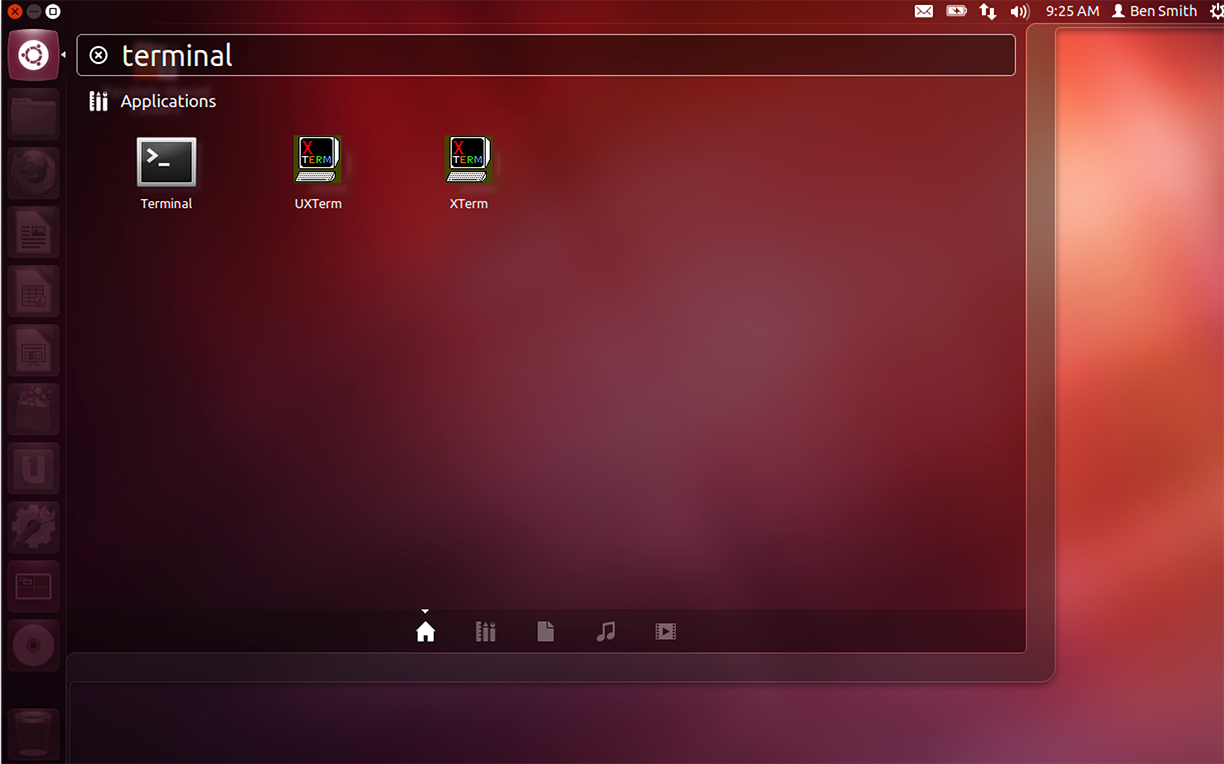
\includegraphics[width=5in]{graphics/OpenTerminal.png}	\caption{Search for terminal app}
\end{figure}

Click on the terminal and type in following. When the terminal asks for your password enter it then press enter:

\begin{quote}
	\begin{verbatim}
		> sudo apt-get install aptitude
	\end{verbatim}
\end{quote}

After you've installed aptitude, make sure to update its database. Type:

\begin{quote}
	\begin{verbatim}
		> sudo aptitude update
	\end{verbatim}
\end{quote}


\section{Install Python with SciPy and Numpy}

The following will install python with all necessary scientific and numeric tools.  Assuming you have installed aptitude and the terminal is open type:

\begin{quote}
	\begin{verbatim}
		> sudo aptitude install python-scipy
	\end{verbatim}
\end{quote}

\section{Install Scrapy}

The following will install python with all necessary tools to scrape websites.  Assuming you have installed aptitude and the terminal is open type:

\begin{quote}
	\begin{verbatim}
		> sudo aptitude install python-scrapy
	\end{verbatim}
\end{quote}

\section{Install LaTeX}

The following will install the base package of LaTeX.  Assuming you have installed aptitude and the terminal is open type:

\begin{quote}
	\begin{verbatim}
		> sudo aptitude install texlive
	\end{verbatim}
\end{quote}

You can have as much or as little of LaTeX installed as you want.  Doing a search for ``texlive" reveals many packages (figure \ref{fig:texlive}).

\begin{quote}
	\begin{verbatim}
		> sudo aptitude search texlive
	\end{verbatim}
\end{quote}
  
\begin{figure}[!h]
	\centering
	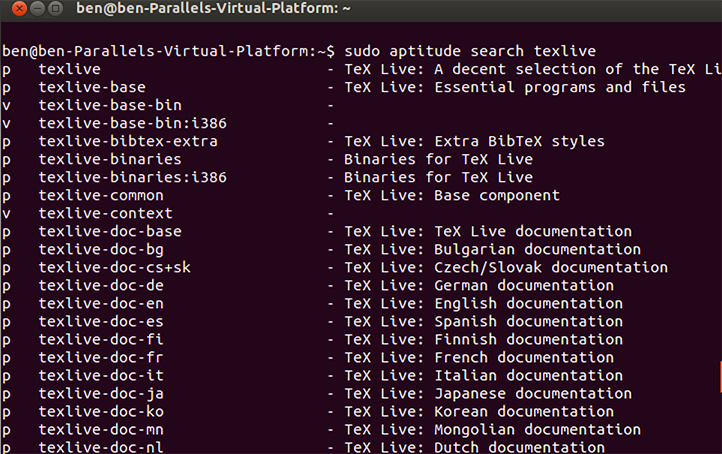
\includegraphics[width=5in]{graphics/ShowTexLivePackages.png}
	\caption{Screenshot of TexLive packages}
	\label{fig:texlive}
\end{figure}

If you wanted to install the extra packages for bibtex, you would type:

\begin{quote}
	\begin{verbatim}
		> sudo aptitude install texlive-bibtex-extra
	\end{verbatim}
\end{quote}

Other packages follow a similar pattern.

\section{Install Kile}

Kile is a LaTeX editor for Linux.  To install Kile, you first need to open the Software Center by searching for ``software":

\begin{figure}[!h]
	\centering
	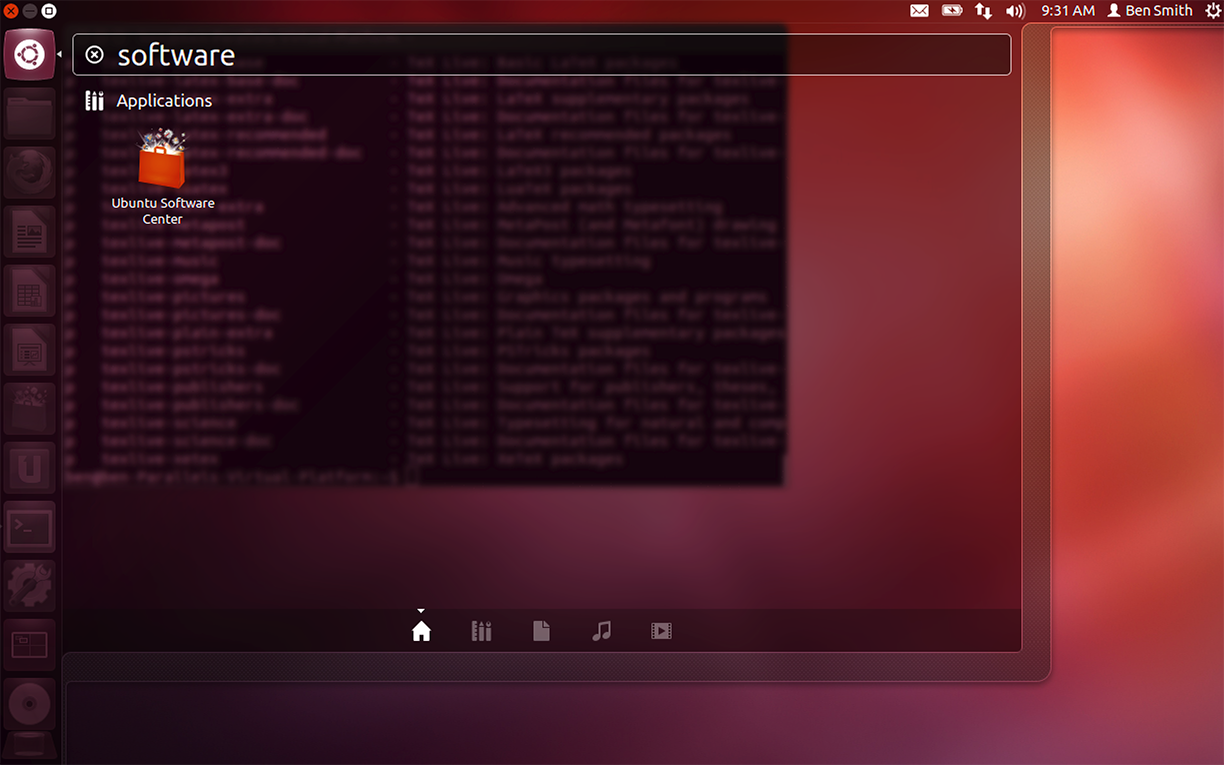
\includegraphics[width=5in]{graphics/OpenSoftwareCenter.png}
	\caption{Search for Software Center}
\end{figure}

From within the Software Center, search for ``Kile":

\begin{figure}[!h]
	\centering
	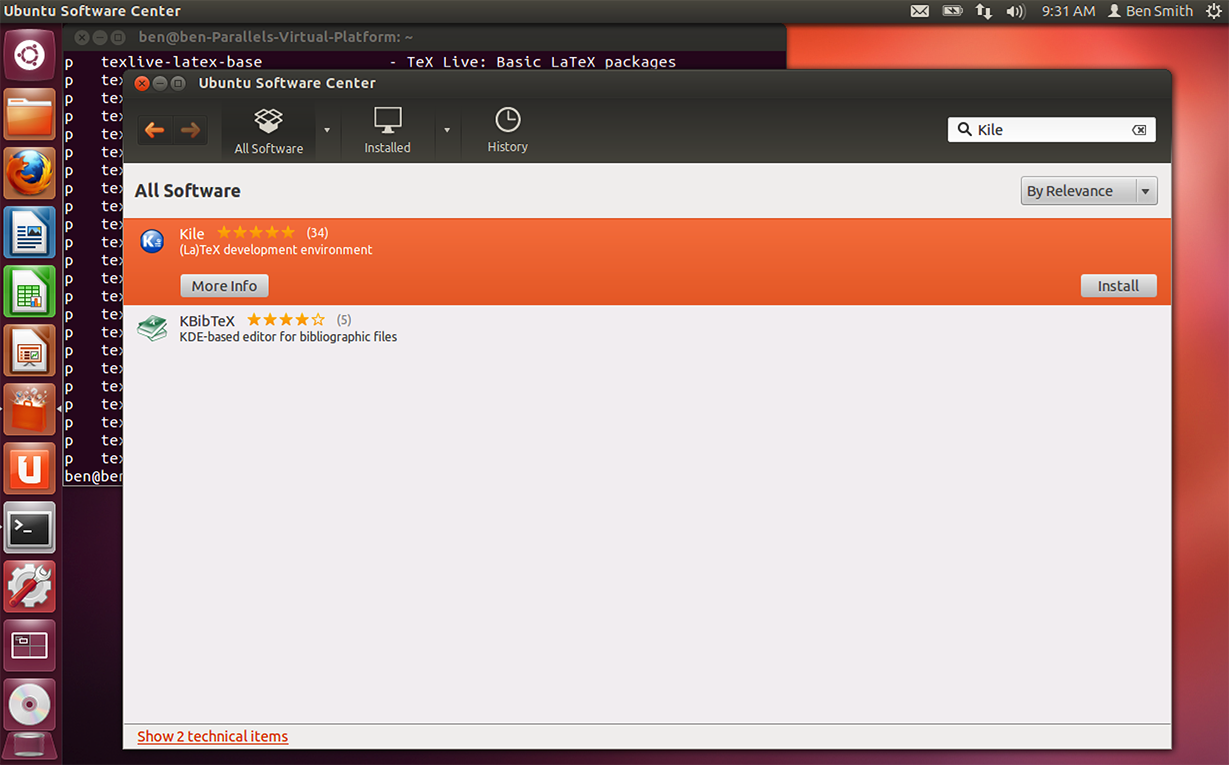
\includegraphics[width=5in]{graphics/FindKile.png}
	\caption{Find ``Kile" in Software Center}
\end{figure}

\vspace{\fill}
\noindent $ \begin{array}{l} \href{http://creativecommons.org/licenses/by/3.0/us/}{
\includegraphics[width=0.25in]{graphics/cc.eps}} \end{array} $ Ben Smith, 2012: \href{http://creativecommons.org/licenses/by/3.0/us/}{Licensed under Creative Commons Attribution 3.0}
\end{document}